\documentclass{article}
\usepackage[utf8]{inputenc}
\usepackage{url}
\usepackage{graphicx}
\graphicspath{ {./} }


\title{Automatisation du prétraitement de photographies de portraits de mandrills}
\author{Maxime Boucher}
\date{Compte rendu 3}

\begin{document}

\maketitle

Pour rappel, l'objectif depuis la dernière fois était d'essayer différents paramètres pour améliorer les résultats sur la classification des photos par qualité. Le but était également de comparer les différentes architectures de base.

\begin{center}
    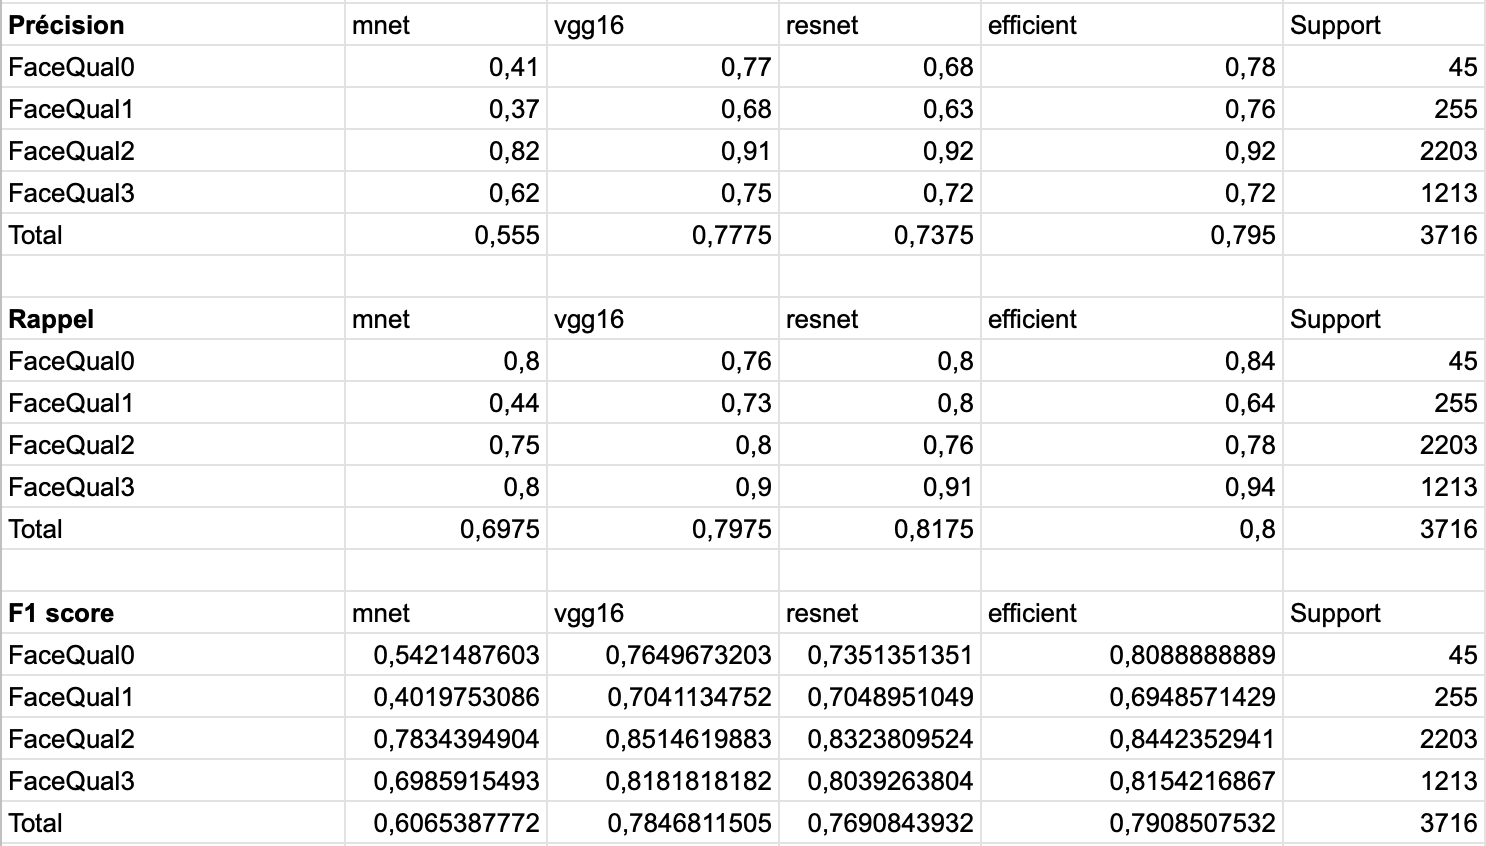
\includegraphics[width=400]{imgs/qualité/cr3/table.png}
\end{center}

\begin{center}
    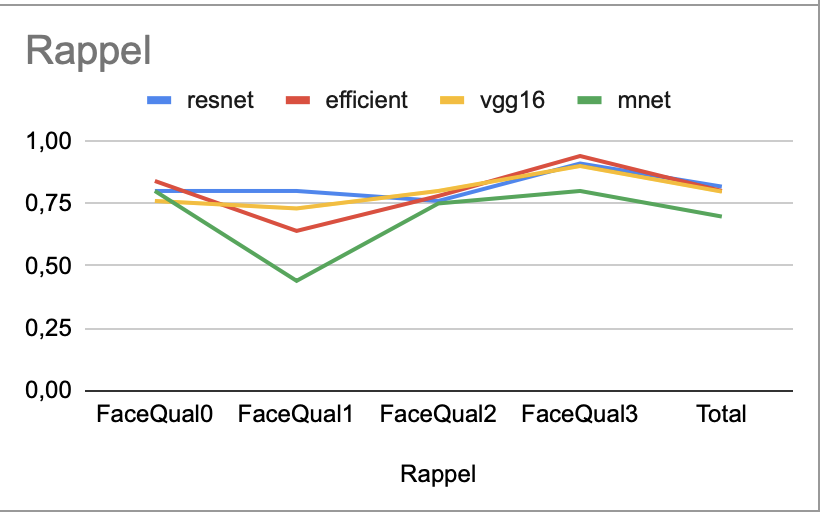
\includegraphics[width=400]{imgs/qualité/cr3/precision.png}
\end{center}
    
Le rappel représente le nombre d'échantillons correctement étiqueté. Ici, l'architecture ResNet prend l'avantage sur la classe FaceQual1 et MobileNet V2 montre de mauvais résultats globaux. Cependant,sur les autres classes EfficientNet prend le dessus.

\begin{center}
    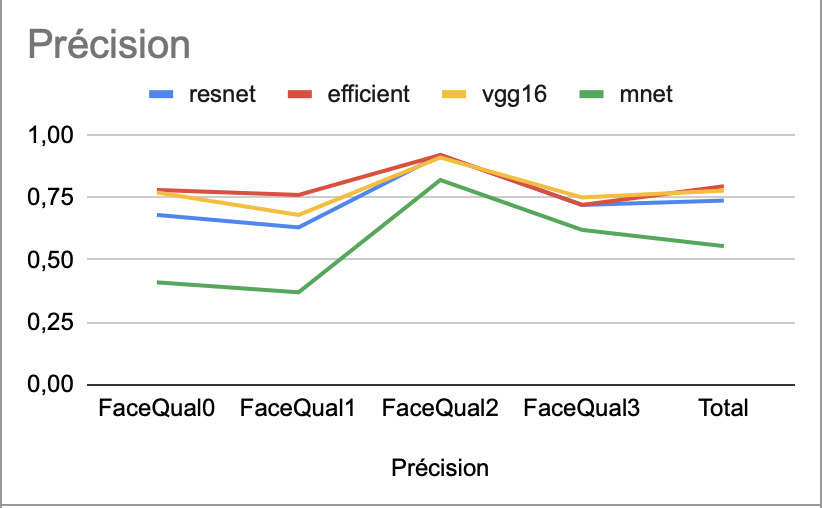
\includegraphics[width=400]{imgs/qualité/cr3/rappel.png}
\end{center}

EfficientNet domine cependant la précision sur pratiquement toutes les classes.

\begin{center}
    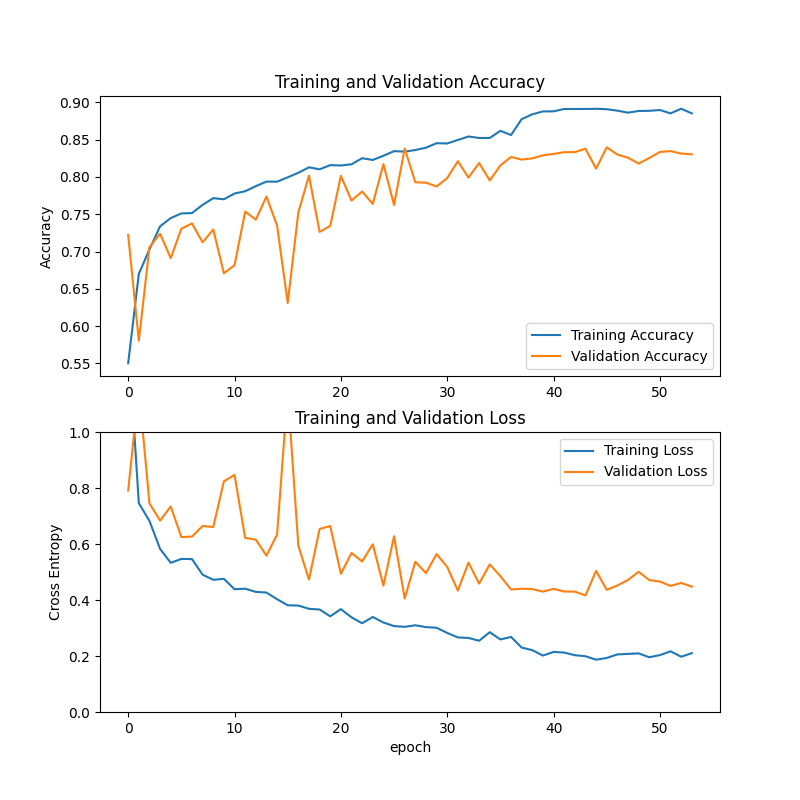
\includegraphics[width=250]{imgs/qualité/cr3/efficient.png}
    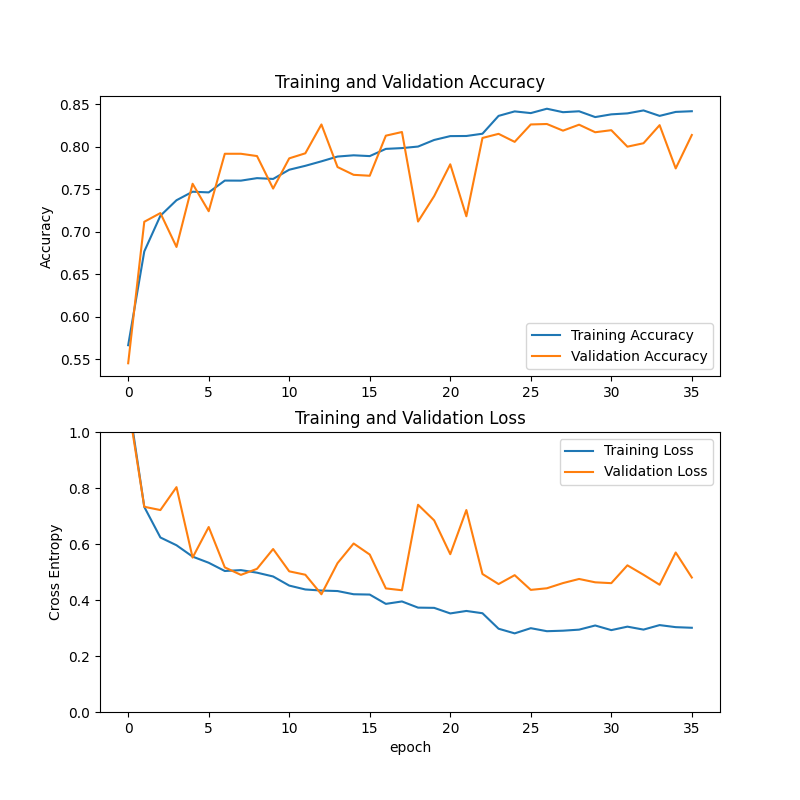
\includegraphics[width=250]{imgs/qualité/cr3/resnet.png}
    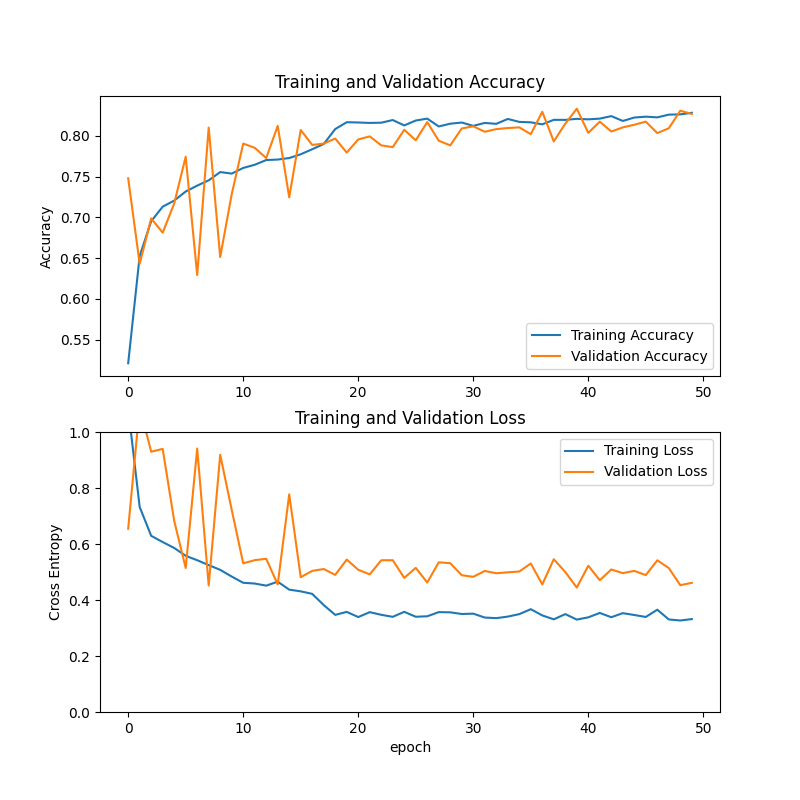
\includegraphics[width=250]{imgs/qualité/cr3/vgg16.png}
\end{center}

Ces trois graphes (efficientnet, resnet, vgg16 dans l'ordre d'apparition) montre que vgg16 obtient les meilleures résultats en regard du surapprentissage mais efficientnet obtient le meilleur score global de validation accuracy.

On va donc maintenant s'intéresser à améliorer le réseau basé sur EfficientNet pour obtenir un résultat encore supérieur. Pour cela, on va d'abord inspecter les images mal classés pour comprendre s'il y a un pattern conduisant à une erreur de classification.

lien du google sheets : https://docs.google.com/spreadsheets/d/1WwJEua33J6X3ySV0A2sB-wlpxmI84EJVIlhFoVNoF20/edit#gid=1842130577

\end{document}
